\subsection{Network Architecture}

The network architecture (\autoref{fig:network}) is based on a basic 3D-UNet implemented by \citeauthor{ronneberger_u-net_2015-1}~\cite{ronneberger_u-net_2015-1} with slight adaptions in downsampling depth, due to memory limitations when using 3D data. We used a downsampling ratio of 8 and a maximum layer depth of 512 in the bottleneck connection. Skip connections are used after each convolutional steps before each pooling layer. To include a multitude of information from the patient aswell as the accelerator, we used five input volumes concatenated along the forth dimension, resulting in an input volume of size $5 \times width \ (W) \times height \ (H) \times depth \ (D)$. As the base resolution for all volmes we used the resolution of our CT scans with voxel dimensions of $1.1718 \times 1.1718 \times 3 mm^3$ in the coronal, sagital, and tanversal plane. 


\begin{figure}
    \centering
    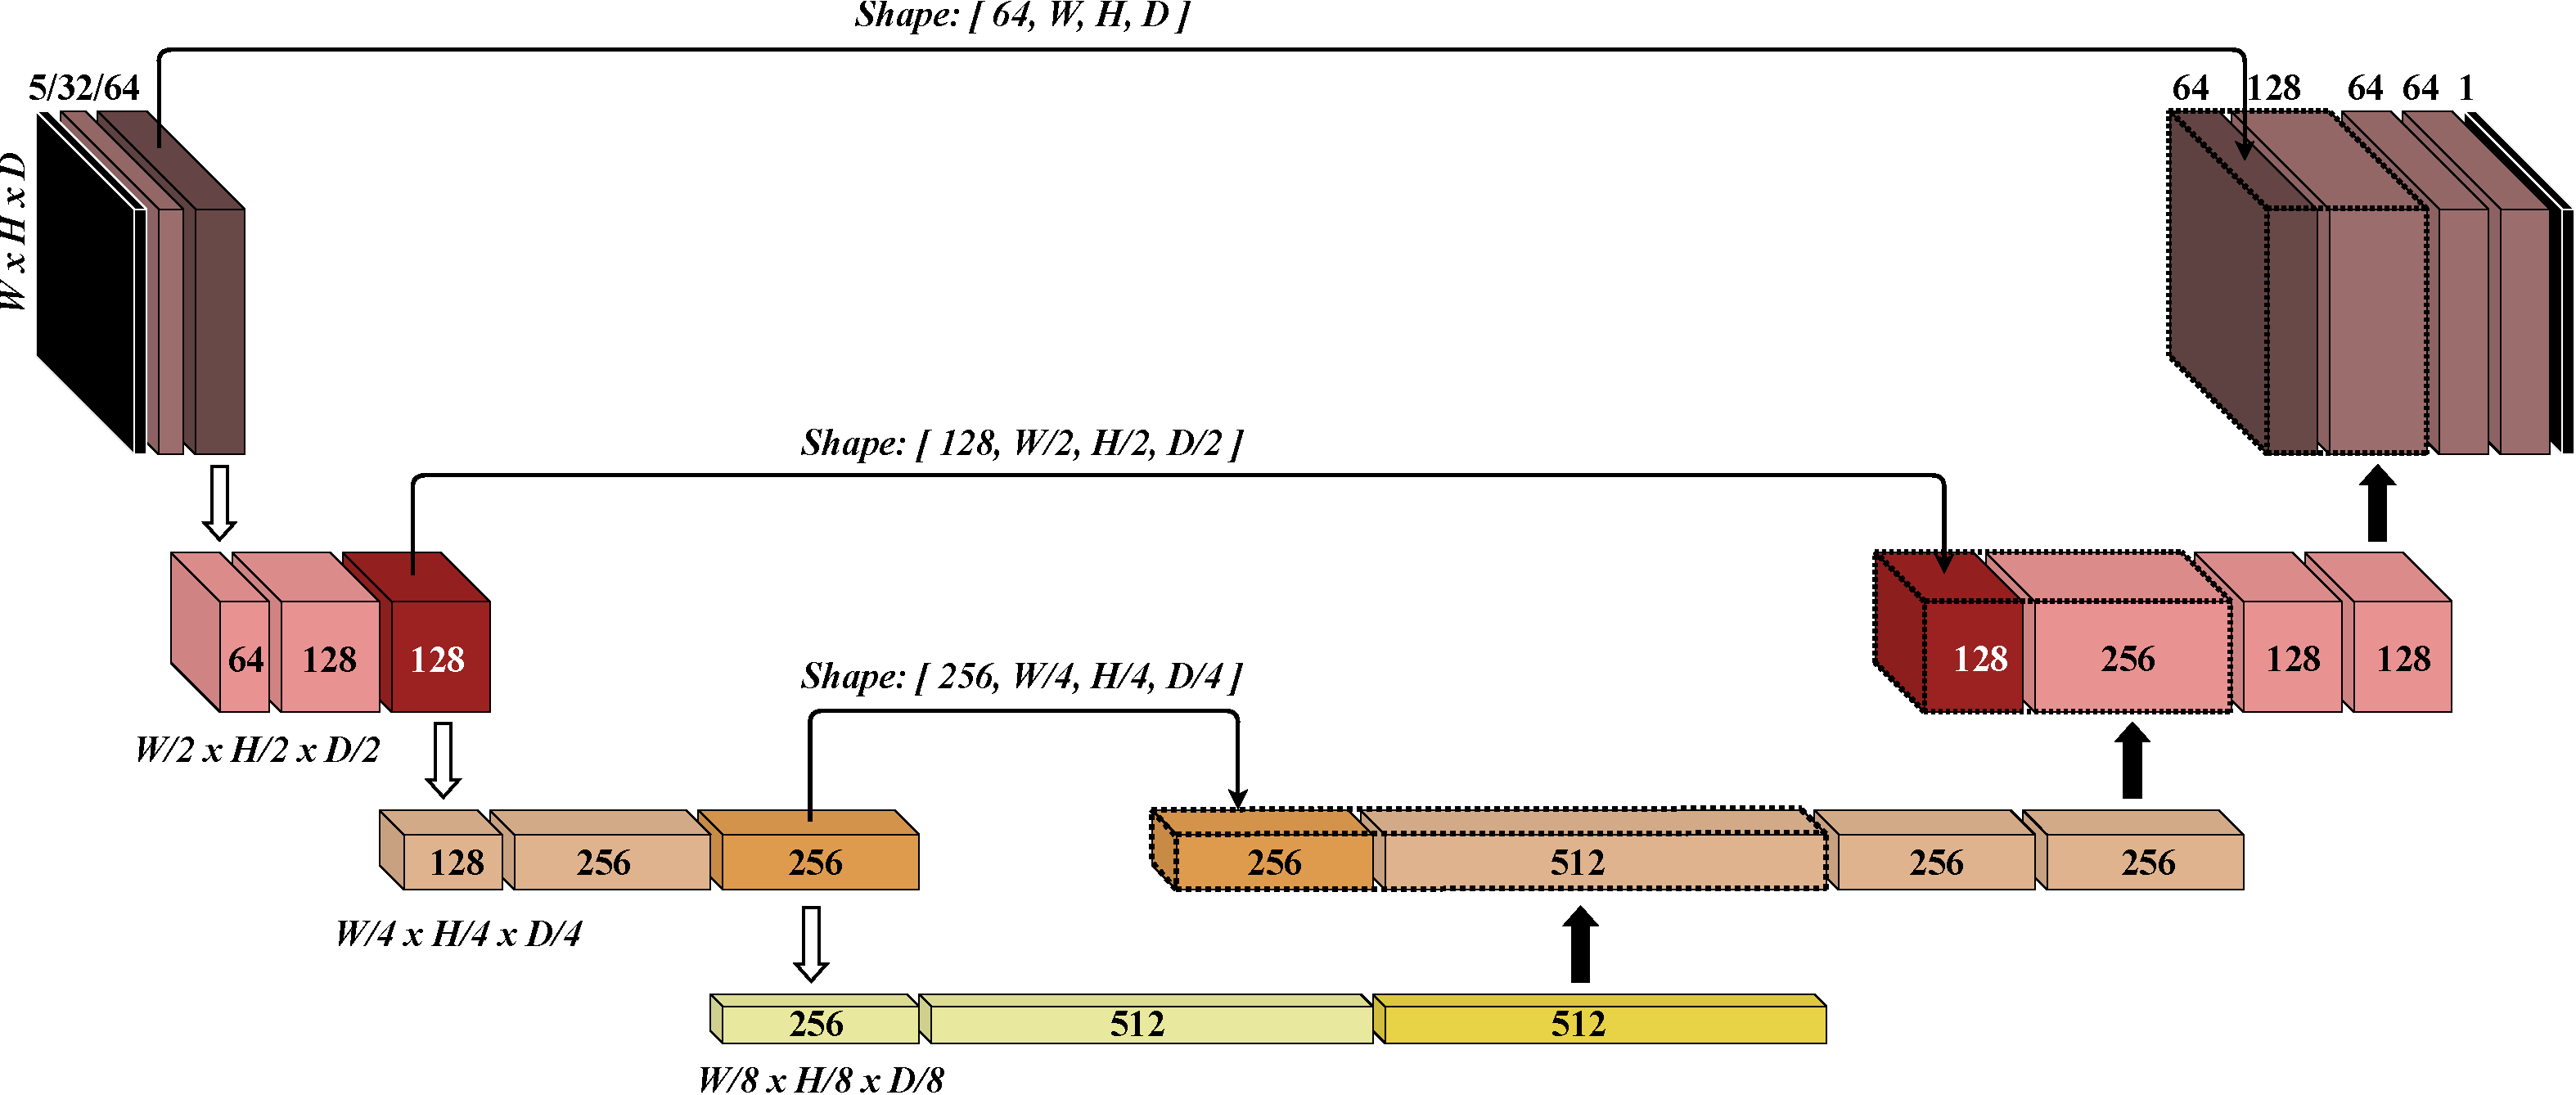
\includegraphics[width=0.9\textwidth]{UNET.pdf}
    \caption{Basic scheme of adapted network architecture with a downsampling ratio of 8 and a maximum depth of 512 in the bottleneck layer. Input dimensions: $5 \times W \times H \times D$; Output dimensions: $1 \times W \times H \times D$}\label{fig:network}
\end{figure}

\subsection{Dataloading}

Memory usage is a serious concern in the application of deep learning and espeacially when dealing with 3D data sets. 
In our case not only the memory usage in the \ac{GPU} but in the \ac{RAM} is of importance. For each training epoch, the network sees all present training data. 
In most applications all data can be loaded into the \acs{RAM} and is then passed onto the \acs{GPU}.
A solution to this problem is to load data on the fly into the RAM and then process it.
This is not applicable because of the immense size of the 3D volumes (multiple 100 MB per volume) that are used for training. 
We therefore developed an partial on the fly dataloading inspired by the \emph{Queue} class from \citeauthor{perez-garcia_torchio_2021}~\cite{perez-garcia_torchio_2021}. 
Due to the quantitative nature of our intput data, we were not able to use data augmentation for our input data. 
To still achieve some additional variation in training data we used the approach of patch based training. 
A multitude of patches can therefore be extracted from the same volume, increasing the variety in training data while using the relatively small number of training volumes. 
To combine the semi-on-the-fly dataloading and the patch based training, multiple volumes are loadded into the RAM and then processed together. 
\autoref{fig:dataloading} shows a scheme of this dataloading approach. 
A fixed amount of training data is loaded from the randomized training data pool and loaded into the RAM. 
From this set of training volumes a subset of patches is extracted from each volume and stored in a queue of patches, which is then shuffled and batch wise passed onto the GPU and the network. 

\begin{figure}
    \centering
    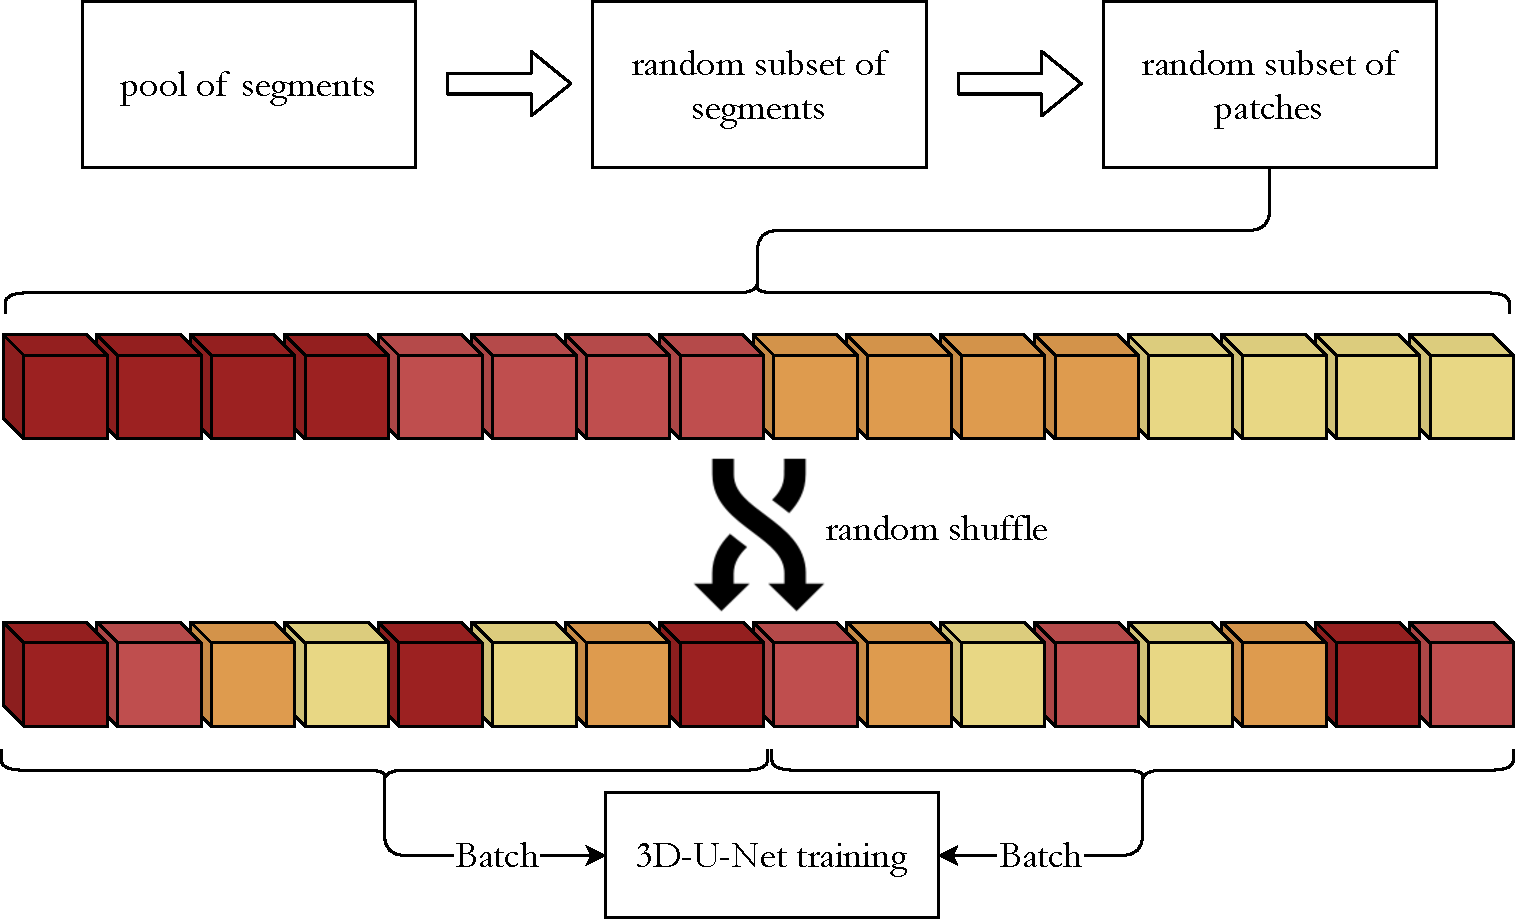
\includegraphics[width=0.7\textwidth]{dataloading.pdf}
    \caption{Dataloading scheme for memory efficient patch based dataloading for 3D training volumes. A subset of patches from one training volume is depicted in one color shade.}\label{fig:dataloading}
\end{figure}

\subsection{Network Input \& Output}

\subsubsection{Network Input}

The network expects five 3D volumes concatenated along their fourth dimension as input. 
These five 3D volumes (\autoref{fig:masks}) combine different spatial, anatomical aswell as accelorator information into the training data. 
By doing so gantry aswell as accelerator head information can be directly translated into 3D space, which makes them interpretable for the network. 

\setlength{\hangingindent}{1em}

\begin{hangingpar}
    \item \textbf{(a) Beam Shape}: The trajectory of the beamshape into 3D space if of crucial importance. 
    It is most important accelerator information for the network. 
    It combines leaf configurations as well as gantry angle into one volume. 
    It acts in some way as a binary indexing mask giving the network information about which voxel is intersected by the beams trajectory into 3D space. 
    To additionaly account for the outputfactor the fieldsize of that specific segment is stored in each voxel intersected by the beam field. 
    The output factor describes the physical process of increasing photon in-scatter into the central beamline for increasing fieldsizes. 
\end{hangingpar}

\begin{hangingpar}
    \item \textbf{(b) Center Beam Line Distance}: The beam of a linear accelerator is best defined in the central beam line. The use of \ac{FF} mostly corrects for this occurence. The distance from the central beam line is therefore of importance for the dose deposition. The minimum distance of each voxel from the central beam line accounting voxel dimensionality is saved in this mask. -> hier mal nochmal drüber reden
\end{hangingpar}

\begin{hangingpar}
    \item \textbf{(c) Source Distance}: 
    The radiation pattern of photons from the accelerator head can be assumed to be the front of a spherical wave. 
    The photon fluence is therefore decreasing with the square of the distance from the source. 
    The source distance mask takes this physical relationship into account. 
    Each voxel within the volume is assigned its distance to the source, taking into account the different voxel dimensions in the different spatial directions. 
    
\end{hangingpar}

\begin{hangingpar}
    \item \textbf{(d) CT}: Dose deposition and particle interaction in genereal are defined by their energy aswell as the electron density of the affected volume. As the energy of the radiated photons is assumed constant, the impact of the electron density of the volume (in this case the patients anatomy) is mainly responsible to the different interaction processes of the photon and secondary electrons. The masks consists of the houndsfield units from the initial CT scan of the patient. Particles radiation from gantry angles below the treatment couch, interact partly inside the treatment couch, therefore it is included in the CT mask. 
\end{hangingpar}

\begin{hangingpar}
    \item \textbf{(e) Radiological Depth}: A photon or electron that passes trough the interaction medium loses its energy on its path. Therefore, the path that a particle follows through a medium is of highly relevant for the dose deposition effects that take place. The radiological depth combines the distance from the source aswell as the interaction mediums density. It is the sum of the path length through a medium multiplied by the density of intersected voxels. Therefore the same spatial depth in a dense material results in a higher radiological depth than the same depth in soft tissue.
\end{hangingpar}

Particles interact negligibly in air, therefore were all masks set to zero where the CT masks was 150 HU over the HU for air. Air or low density volumes inside the body of the patient were not affected by this step, to account for the \ac{ERE} on the surface of air cavities inside the patient. 

\begin{figure}
    \centering
    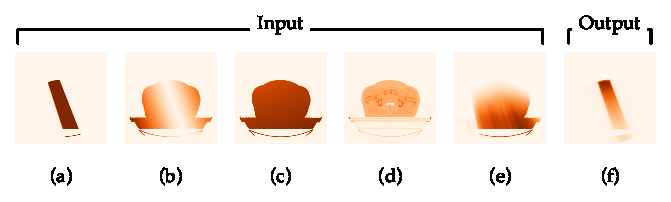
\includegraphics[width=\textwidth]{masks.pdf}
    \caption{Examplary input and output for a single segment of a prostate plan. (a): beam shape, (b): center beam line distance, (c): source distance, (d): CT, (e): radiological depth, (f): dose distribution, }\label{fig:masks}
\end{figure}

\subsubsection{Network Output}

The network combines the information from the five 3D volumes and yields a single volume with the respective dose distribution for the given input. Spatial dimensions for width height and depth aswell as voxel dimensions are preserved during inference. In \autoref{fig:masks} (f) an exemplary dose distribution for the respective inputs (a) - (e) is given

\subsection{Training Data Generation}

All training data was generated from patient data taken from the institutional database of radiotherapy treatment plans. 
Information for all input masks are given in the CT scan, the dose file aswell as the plan file. 
The patients anatomy for the CT masks is taken from the CT files and adjusted to the right slice thickness, due to different aquisition protocols using 2~mm or 3~mm slice spacing. 
Dose distribution used as training target for each segment were calculated using the EGSnrc open source software package provided under~\cite{noauthor_nrc-cnrcegsnrc_2021}. 
The work of \citeauthor{friedel_development_2019} enabled us to accurately simulate single segment dose distributions for the MR-Linac. 
Simulation of all segments was dose using a remote \ac{HPC} solution provided by the state of Baden-Württemberg. 
Coordinate system orientation of the patients anatomy as well as \ac{MLC} and gantry positions are given in the dose and plan file. 
Simulation of $10^7$ particles took around 4 hours on average.
The 3D input volumes to the network were calculated using in-house developed python scripts with the provided information from CT, dose and plan files. (GITHUB LINK?, hier noch näher drauf eingehen?)

\subsection{Evaluation Metrics}

Dose conformaty of dose distributions are clinically assessed using the gamma-index metric first introduced by \citeauthor{low_technique_1998}~\cite{low_technique_1998} in \citeyear{low_technique_1998}. The evaluation metric composed of two parametric values that set the criteria for which dose distributions are analysed. Spatial deviations aswell as deviations of dose are respected when analysing. Dose conformaty is assessed by analyzing each individual voxel of a given dose distribution using the following equation:

\begin{equation}\label{eq:gamma}
    \Gamma (r_m, r_c) = \sqrt{\frac{r^2(r_m,r_c)}{\Delta d^2_M} + \frac{\delta ^2(r_m,r_c)}{\Delta D^2_M}}
\end{equation}

where $\Delta D_M$ and $\Delta d_M$ are the dose difference and spatial criterion respectively, in our case 3\% and 3~mm.  $r^2(r_m,r_c)$ and $\delta ^2(r_m,r_c)$ are the squared spatial distance and dose difference from the reference point $r_m$ to evaluation point $r_c$ respetively. If $\Gamma \leq 1$ the criterion are passed. By evaluating the entire volume in that manner an overrall gamma passrate can be calulated with the following formula. 

\begin{equation}\label{eq:gamma_rate}
    \gamma = \frac{NoT(\Gamma \leq 1)}{NoT}
\end{equation}

where $NoT$ is the number of points to be tested, in this case the number of voxels in the entire volume and $NoT(\Gamma \leq 1)$ is the number of tests that passed the gamma criterion following \autoref{eq:gamma}. The equations \autoref{eq:gamma} and \autoref{eq:gamma_rate} hold true for single aswell as multiple dimensions. A 2D example for a passed aswell as a failed gamma test is given in \autoref{fig:gamma}. 

\begin{figure}
    \centering
    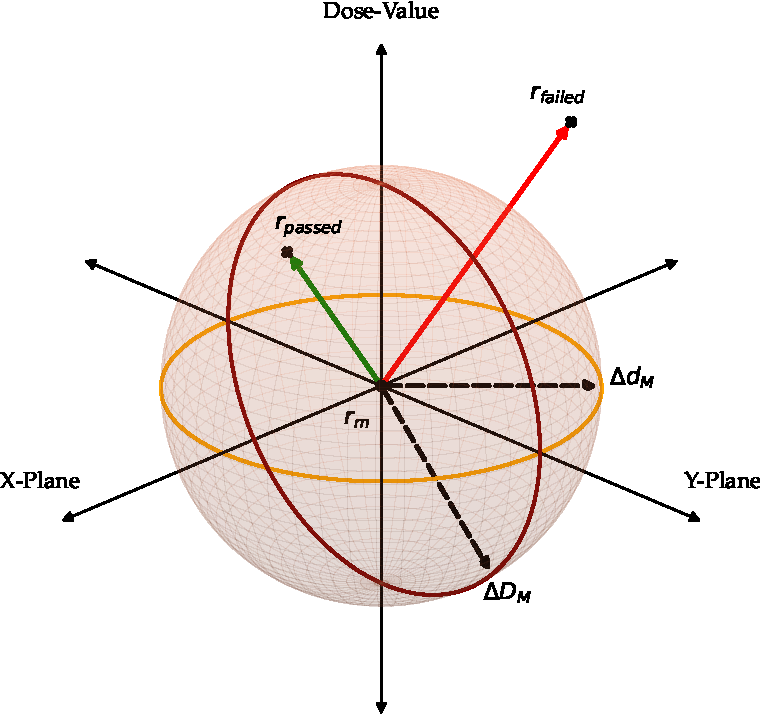
\includegraphics[width=0.5\textwidth]{gamma.pdf}
    \caption{Gamma test for two points $r_{passed}$ and $r_{failed}$ and the reference point $r_m$ for a 2D (X,Y) space case. Orange and brown rings indicate distance and dose parameter acceptance margins respectively. The Gray sphere represents the set of all points that pass the gamma test. Green and Red arrow indicate a passed and failed gamma test for the given reference point $r_m$, dose and spatial parameter.}\label{fig:gamma}
\end{figure}

\subsection{Hypotheses and Experiments}

\subsubsection{General Applicability}\label{sssec:H1}
\begin{hanginglist}\itemsep2pt

    \item\textbf{Hypothesis}\newline
    The network is able to learn the general dose deposition process from the given input taken from a multitude of radio treatment segments of one tumor entity. 
    Dose predictions for segments of the same entity are accurate and robust.

    \item\textbf{Experiment}\newline
    Training of the proposed 3D-UNet on a mutlitude of prostate cancer patient radio treatment segments. 
    Dose conformaty assessment with the gamma passrate for each individual test segment aswell as entire test plans. 

\end{hanginglist}

\subsubsection{Poor Initial Translatability}\label{sssec:H2}
\begin{hanginglist}\itemsep2pt

    \item\textbf{Hypothesis}\newline
    Different tumor sites vary drastically in segment shape, orientation and \ac{SSD}. The \acs{SSD} is, compared to other entities such as \acs{HN}, mostly constant for prostate cancer patients. The same holds true for tissue homogenity aspects of the respective body regions, when comparing lower abdomen to e.g. \acs{HN}. We therefore assume that the network will not reach the previously achieved gamma passrates when testing on different tumor sites and patient anatomies. 

    \item\textbf{Experiment}\newline
    The from \emph{\ref{sssec:H1} \nameref{sssec:H1}} trained network is then used for inference on additional testing data from a multitude of tumor entities aswell as patient anatomies to test its translational capabilities to a varying set of input characteristics. 

\end{hanginglist}

\subsubsection{Increased Robustness}\label{sssec:H3}
\begin{hanginglist}\itemsep2pt

    \item\textbf{Hypothesis}\newline
    The includation of a broader variety of segments shapes, sizes and positions inside the patients anatomy, as well as differing body regions and therefore varying \acs{SSD} values and tissue densities result in a better robustness of the networks prediction accuracy. 

    \item\textbf{Experiment}\newline
    Network architecture aswell as training algorithm of the in \emph{\ref{sssec:H1} \nameref{sssec:H1}} trained network are kept, while including additional trainign data from liver, breast and \acs{HN} patients. 
    We therefore include liver, breast and \ac{HN} into the training of the same network from \emph{Hypothesis 1}. The translational capabilities are then assed by testing the newly trained network on prostate, liver, breast, H\&N and lymph node data. By doing this we asses if the network performance decreases on prostate data by including new tumor sites into the training data and we assess its performance on seen (prostate, liver, heaad \& neck, breast) aswell as unseen treatment plan data (lymph nodes).

    \item\textbf{Experiment}:
\end{hanginglist}

\subsubsection{Underlying Physics}\label{sssec:H4}
\begin{hanginglist}\itemsep2pt
    \item\textbf{Hypothesis 4}: The network is capable of learning the underlying physics of the dose depositiopn process. 
    \item\textbf{Experiment 4}: in order to decouple the dose delivery from the patient anatomy, we have created a phantom data set. The phantoms consist of an air volume in the shape of a cube with the dimensions 600 $\times$ 600 $\times$ 600 $mm^3$ (512 $\times$ 512 $\times$ 200 voxel for coronal, sagital and transversal plane, respectively). Within this air volume, a water slab is placed at various locations to account for the influence of the distance-squared law. in this volume, we now simulate and predict a 10 $\times$ 10 beam from 0° and observe the depth dose profile, as well as the coronal and sagital transverse dose profiles in the middle of the water volume. A multitude of aspects of the physics can distance-squared law, penumbra, qualitative and quantitative depth dose profiles, field divergence in central beamline. 
\end{hanginglist}

\subsection{Patient Data}
All patients gave their informed written consent to this study, which was approved by the local ethical committee (ethics approval No. 659/2017BO1).
patient data from our institution previously treated at the mr linac.\ all plans were created by a medical physicist in agreement with a oncologist
Welche Entitäten: Prostate only training: 45 prostate treatment plans with a total of 2342 Segments, 36/4/5 split für train / val / test split.\ with a mean fieldsize of 36.57 ± 17.9 cm\textsuperscript{2} for training / validation set and 34.57 ± 15.86 cm\textsuperscript{2} for the test set.
mixed model 15 prostate with 720 segments, 35.49 ± 18.01 and 34.57 ± 15.86 15 liver 819 Segments 24.09 ± 18.36 and 22.81 ± 14.47 15 mamma 656 Segments 40.72 ± 28.48 and 40.60 ± 37.98 14 head \& neck 929 segments in einem 8/2/5 split also in 32/8/20 train / validation / test ratio.\ aswell as 15 patient plans 659 segments for lymphnodes exclusively for testing with a mean fieldsize of 25.95 ± 25.59
as you can see in \autoref{tab:patients}
All patients gave their informed written consent to this study, which was approved by the local ethical committee (ethics approval No. 659/2017BO1).


\begin{table}
\centering
    \scalebox{0.7}{
        \begin{tabular}{|lcccccc|}
        \hline
                                            & \textbf{Prostate-Only}           & \multicolumn{4}{c}{\textbf{Mixed-Entity}}                                   & \textbf{Testing} \\ \hline
                                            & \multicolumn{1}{c|}{}            & Liver       & Mamma       & Head \& Neck & \multicolumn{1}{c|}{Prostate}    & Lymphnodes       \\
            Number of Patients              & \multicolumn{1}{c|}{45}          & 15          & 15          & 15           & \multicolumn{1}{c|}{15}          & 15               \\
            Number of Segments              & \multicolumn{1}{c|}{2342}        & 819         & 656         & 929          & \multicolumn{1}{c|}{720}         & 659              \\
            Training / Validation / Testing & \multicolumn{1}{c|}{36/4/5}      & 8/2/5       & 8/2/5       & 8/2/5        & \multicolumn{1}{c|}{8/2/5}       & Only Testing     \\
            Fieldsize Training/Validation   & \multicolumn{1}{c|}{36.5 (17.9)} & 24.1 (18.4) & 40.7 (28.5) & 63.0 (50.5)  & \multicolumn{1}{c|}{35.5 (18.0)} & N/A              \\
            Fieldsize Testing               & \multicolumn{1}{c|}{34.5 (15.8)} & 22.8 (14.4) & 40.6 (38.0) & 68.9 (53.6)  & \multicolumn{1}{c|}{34.6 (15.9)} & 26.0 (25.6)      \\ \hline
        \end{tabular}
    }
    \caption{Patient data infortmation for Prostate-Only as well as Mixed-Entity trained model and testing data set. Fieldsizes are given as mean (standard deviation).}\label{tab:patients}
\end{table}
